%% The first command in your LaTeX source must be the \documentclass command.
%%
%% Options:
%% twocolumn : Two column layout.
%% hf: enable header and footer.
\documentclass[
% twocolumn,
% hf,
]{ceurart}

%%
%% One can fix some overfulls
% \sloppy

%%
%% Minted listings support
%% Need pygment <http://pygments.org/> <http://pypi.python.org/pypi/Pygments>
\usepackage{minted}
%% auto break lines
\setminted{breaklines=true}
\usepackage{doi}
\def\doitext{DOI:}
% \newcommand{\doi}[1]{DOI:#1}

%%
%% end of the preamble, start of the body of the document source.
\begin{document}

%%
%% Rights management information.
%% CC-BY is default license.
\copyrightyear{2021}
\copyrightclause{Copyright for this paper by its authors.
  Use permitted under Creative Commons License Attribution 4.0
  International (CC BY 4.0).}

%%
%% This command is for the conference information
\conference{ITAMS'2021: Information Technologies: Algorithms, Models, Systems. September 17${}^{th}$, 2021, Irkutsk, Russia}

%%
%% The "title" command
\title{Web-GIS viewer for active faults data represented as a knowledge graph}

%%
%% The "author" command and its associated commands are used to define
%% the authors and their affiliations.
\author[1,3,4]{Evgeny A. Cherkashin}[%
orcid=0000-0003-2428-2471,
email=eugeneai@icc.ru,
url=https://github.org/eugeneai,
]
\address[1]{Matrosov Institute for System Dynamics and Control Theory of Siberian Branch of Russian Academy of Sciences, 134 Lermontov St, Irkutsk, 664033, Russian Federation}

\author[2]{Oksana V. Lunina}[%
orcid=0000-0001-7743-8877,
email=lounina@crust.irk.ru,
url=http://www.crust.irk.ru/member_88.html,
]

\address[2]{Institute of the Earth’s Crust of Siberian Branch of Russian Academy of Sciences, 128 Lermontov St, Irkutsk, 664033, Russian Federation}

\author[3]{Leonid O. Demyanov}

\address[3]{Institute for Mathematics and Informational Technologies, Irkutsk State University, 20~Gagarina Bulv, Irkutsk, 664003, Russian Federation}

\author[4]{Alexander V. Tsygankov}

\address[4]{Institute for Information Technologies and Data Analysis, National Research Irkutsk State Technical University, 83~Lermontov St, Irkutsk, 664074, Russian Federation}

%%
%% The abstract is a short summary of the work to be presented in the
%% article.
\begin{abstract}
  A problem of flexible geographical data representation and Web-based visualization is considered.  The data stored in a knowledge graph as ontologies (vocabularies) in accordance to W3C standards.  For viewing data, a web geographical information system (GIS) application is realized, which renders map interpreting SPARQL queries to Sematic Web server storing the knowledge graph.  The technologies used for designing are based on contemporary Web 3.0, allowing one to implement Linked Open Data compliance for GIS information publishing and integration.
\end{abstract}

%%
%% Keywords. The author(s) should pick words that accurately describe
%% the work being presented. Separate the keywords with commas.
\begin{keywords}
  geographical information system \sep
  knowledge graph \sep
  semantic web \sep
  storing flexible data \sep
  one-page web application
\end{keywords}

%%
%% This command processes the author and affiliation and title
%% information and builds the first part of the formatted document.
\maketitle

\section{Introduction}

Contemporary Web technologies development is aimed at more tight data integration: standardization of data publishing formats, formal data and metadata representation, modeling interpretation contexts.  Geospatially related objects are frequently published as well.

In this investigation the fault data are chosen as subject for representation and publishing.  Geological field investigations and event observations, \emph{e.g.}, earthquakes, accumulate data, which are analyzed, resulting in setting new attributes to a fault or their refinement.  According to the techniques of geological research additional information are associated with attributes clarifying their values.  Such clarification comprises precision characteristics, measurement conditions, reliability assessment, and paper references, where fault data were published.

GIS\footnote{Abbreviation of Geographical Information System} represents spatial data in semantic defined layers.  For each object of a layer, one can associate a set of attribute values of auxiliary data.  The set of the attributes are the same for each object of the layer regardless of wether the attribute value is defined for an object or not.  Empty values are represented as ``\texttt{null}''s.  In the case of geological exploration, when a lot of attributes are undefined, this approach leads to sparse filled tables.  This, in turn, requires data modification and analysis algorithms to utilize additional data checking stages when using standard relation operations (SELECT, UPDATE, DELETE).

Another question is attribute names definition expressing semantics of metadata.  For example, to define a precision of a value one could construct an attribute name with ``\texttt{\_prec}'' suffix, where name is its value attribute identifier.  Other types of metadata add more suffixes, as well as relations between suffixes and values are not defined anywhere in database.  The formal definition is to be defined in a documentation or processing algorithms, thus, either informally defined or obfuscated, and practically not alienated.  Adding new attributes requires user to devise new synthetic names.

Web publication applications, as information systems, are to implement filtering functions, differentiating the value attributes and their metadata.  Screen widgets label names either defined in application or figured out from the attribute names.  Lack of ontological (vocabulary) formal domain definition forces developer to spend more efforts for user interface implementation.

Since 2001 Semantic Web technologies have evolved in a substantial set of instruments for data storing, publishing, and software integration, allowing system designers and programmers, among standard means, pass data between systems via published documents and application user interfaces, \emph{i.e.}, extending their set of functions.  Vocabularies and data instances are stored in graph databases, which provide SPARQL and other endpoints on top of HTTP protocols, enabling similar services as relational database servers for data access and modification.  The generalized problem statements and approaches to their solutions in the field of Semantic Web are the reasons of its constant development.

Knowledge graphs (KG) \cite{hogan} are techniques of Sematic Web usage aimed at representation data in a general flexible way allowing so-called ``natural'' evolving of domain image, including representation of incomplete knowledge.  This evolution correspond to a scientific research process, where data is accumulated and analyzed.  KG enables both providing in addition distributed storage, federated query based access and modification, means for metadata definition, and formalized verification of its content.

The aim of this research and development is to represent existing tabular and spatial data from \cite{lunina,afs} as a knowledge graph with implementing a viewer, assessing ``working efficiency'' of a programmer and ``usability'' of KG services.  State further development perspectives, ranging them by priorities.

\section{Data conversion}

\section{Viewer implementation}

\section{Examples of usage}

\section{Related Works}

\section{Future activity plan}

\section{Conclusion}


CEUR-WS's article template provides a consistent \LaTeX{} style for
use across CEUR-WS publications, and incorporates accessibility and
metadata-extraction functionality. This document will explain the
major features of the document class % \footnote{You can use this
%  document as the template for preparing your publication. We
%  recommend using the latest version of the ceurart style.
%}.

If you are new to publishing with CEUR-WS, this document is a valuable
guide to the process of preparing your work for publication.

The ``\verb|ceurart|'' document class can be used to prepare articles
for any CEUR-WS publication, and for any stage of publication, from
review to final ``camera-ready'' copy with {\itshape very} few changes
to the source.

This class depends on the following packages
for its proper functioning:

\begin{itemize}
\item \verb|natbib.sty| for citation processing;
\item \verb|geometry.sty| for margin settings;
\item \verb|graphicx.sty| for graphics inclusion;
\item \verb|hyperref.sty| optional package if hyperlinking is required in
  the document;
\item \verb|fontawesome5.sty| optional package for bells and whistles.
\end{itemize}

All the above packages are part of any
standard \LaTeX{} installation.
Therefore, the users need not be
bothered about downloading any extra packages.

\section{Modifications}

Modifying the template --- including but not limited to: adjusting
margins, typeface sizes, line spacing, paragraph and list definitions,
and the use of the \verb|\vspace| command to manually adjust the
vertical spacing between elements of your work --- is not allowed.

\section{Template parameters}

There are a number of template
parameters which modify some part of the \verb|ceurart| document class.
This parameters are enclosed in square
brackets and are a part of the {\verb|documentclass|} command:
\begin{minted}{latex}
  \documentclass[parameter]{ceurart}
\end{minted}

Frequently-used parameters, or combinations of parameters, include:
\begin{itemize}
\item {\verb|twocolumn|}: Two column layout.
\item {\verb|hf|}: Enable header and footer\footnote{You can enable
    the display of page numbers in the final version of the entire
    collection. In this case, you should adhere to the end-to-end
    pagination of individual papers.}.
\end{itemize}

\section{Front matter}

\subsection{Title Information}

The titles of papers should be either all use the emphasizing
capitalized style or they should all use the regular English (or
native language) style. It does not make a good impression if you or
your authors mix the styles.

Use the \verb|\title| command to define the title of your work. Do not
insert line breaks in your title.

\subsection{Title variants}

\verb|\title| command have the below options:
\begin{itemize}
\item \verb|title|: Document title. This is default option.
\begin{minted}{latex}
\title[mode=title]{This is a title}
\end{minted}
You can just omit it, like as follows:
\begin{minted}{latex}
\title{This is a title}
\end{minted}

\item \verb|alt|: Alternate title.
\begin{minted}{latex}
\title[mode=alt]{This is a alternate title}
\end{minted}

\item \verb|sub|: Sub title.
\begin{minted}{latex}
\title[mode=sub]{This is a sub title}
\end{minted}

\item \verb|trans|: Translated title.
\begin{minted}{latex}
\title[mode=trans]{This is a translated title}
\end{minted}

\item \verb|transsub|: Translated sub title.
\begin{minted}{latex}
\title[mode=transsub]{This is a translated sub title}
\end{minted}
\end{itemize}

\subsection{Authors and Affiliations}

Each author must be defined separately for accurate metadata
identification. Multiple authors may share one affiliation. Authors'
names should not be abbreviated; use full first names wherever
possible. Include authors' e-mail addresses whenever possible.

\verb|\author| command have the below options:

\begin{itemize}
\item \verb|style|: Style of author name (chinese)
\item \verb|prefix|: Prefix
\item \verb|suffix|: Suffix
\item \verb|degree|: Degree
\item \verb|role|: Role
\item \verb|orcid|: ORCID
\item \verb|email|: E-mail
\item \verb|url|: URL
\end{itemize}

Author names can have some kinds of marks and notes:
\begin{itemize}
\item affiliation mark: \verb|\author[<num>]|.
% \item email: \verb|\ead{<email>}|,
% \item url: \verb|\ead[url]{<url>}|.
\end{itemize}

The author names and affiliations could be formatted in two ways:
\begin{enumerate}
\item Group the authors per affiliation.
\item Use an explicit mark to indicate the affiliations.
\end{enumerate}

Author block example:
\begin{minted}{latex}
\author[1,2]{Author Name}[%
    prefix=Prof.,
    degree=D.Sc.,
    role=Researcher,
    orcid=0000-0000-000-0000,
    email=name@example.com,
    url=https://name.example.com
]

\address[1]{Affiliation #1}
\address[2]{Affiliation #2}
\end{minted}

\subsection{Abstract and Keywords}

Abstract shall be entered in an environment that starts
with \verb|\begin{abstract}| and ends with
\verb|\end{abstract}|.

\begin{minted}{latex}
\begin{abstract}
  This is an abstract.
\end{abstract}
\end{minted}

The key words are enclosed in a \verb|{keyword}|
environment. Use \verb|\sep| to separate keywords.

\begin{minted}{latex}
\begin{keywords}
  First keyword \sep
  Second keyword \sep
  Third keyword \sep
  Fourth keyword
\end{keywords}
\end{minted}

At the end of front matter add \verb|\maketitle| command.

\section{Sectioning Commands}

Your work should use standard \LaTeX{} sectioning commands:
\verb|section|, \verb|subsection|, \verb|subsubsection|, and
\verb|paragraph|. They should be numbered; do not remove the numbering
from the commands.

Simulating a sectioning command by setting the first word or words of
a paragraph in boldface or italicized text is not allowed.

\section{Tables}

The ``\verb|ceurart|'' document class includes the ``\verb|booktabs|''
package --- \url{https://ctan.org/pkg/booktabs} --- for preparing
high-quality tables.

Table captions are placed \textit{above} the table.

Because tables cannot be split across pages, the best placement for
them is typically the top of the page nearest their initial cite.  To
ensure this proper ``floating'' placement of tables, use the
environment \verb|table| to enclose the table's contents and the
table caption. The contents of the table itself must go in the
\verb|tabular| environment, to be aligned properly in rows and
columns, with the desired horizontal and vertical rules.

Immediately following this sentence is the point at which
Table~\ref{tab:freq} is included in the input file; compare the
placement of the table here with the table in the printed output of
this document.

\begin{table*}
  \caption{Frequency of Special Characters}
  \label{tab:freq}
  \begin{tabular}{ccl}
    \toprule
    Non-English or Math&Frequency&Comments\\
    \midrule
    \O & 1 in 1,000& For Swedish names\\
    $\pi$ & 1 in 5& Common in math\\
    \$ & 4 in 5 & Used in business\\
    $\Psi^2_1$ & 1 in 40,000& Unexplained usage\\
  \bottomrule
\end{tabular}
\end{table*}

To set a wider table, which takes up the whole width of the page's
live area, use the environment \verb|table*| to enclose the table's
contents and the table caption.  As with a single-column table, this
wide table will ``float'' to a location deemed more
desirable. Immediately following this sentence is the point at which
Table~\ref{tab:commands} is included in the input file; again, it is
instructive to compare the placement of the table here with the table
in the printed output of this document.

\begin{table}
  \caption{Some Typical Commands}
  \label{tab:commands}
  \begin{tabular}{ccl}
    \toprule
    Command &A Number & Comments\\
    \midrule
    \texttt{{\char'134}author} & 100& Author \\
    \texttt{{\char'134}table}& 300 & For tables\\
    \texttt{{\char'134}table*}& 400& For wider tables\\
    \bottomrule
  \end{tabular}
\end{table}

\section{Math Equations}

You may want to display math equations in three distinct styles:
inline, numbered or non-numbered display.  Each of the three are
discussed in the next sections.

\subsection{Inline (In-text) Equations}

A formula that appears in the running text is called an inline or
in-text formula.  It is produced by the \verb|math| environment,
which can be invoked with the usual
\verb|\begin| \ldots \verb|\end| construction or with
the short form \verb|$| \ldots \verb|$|. You can use any of the symbols
and structures, from $\alpha$ to $\omega$, available in
\LaTeX~\cite{Lamport:LaTeX};
this section will simply show a few
examples of in-text equations in context. Notice how this equation:
\begin{math}
  \lim_{n\rightarrow \infty} \frac{1}{n} = 0,
\end{math}
set here in in-line math style, looks slightly different when
set in display style.  (See next section).

\subsection{Display Equations}

A numbered display equation---one set off by vertical space from the
text and centered horizontally---is produced by the \verb|equation|
environment. An unnumbered display equation is produced by the
\verb|displaymath| environment.

Again, in either environment, you can use any of the symbols and
structures available in \LaTeX{}; this section will just give a couple
of examples of display equations in context.  First, consider the
equation, shown as an inline equation above:
\begin{equation}
  \lim_{n\rightarrow \infty} \frac{1}{n} = 0.
\end{equation}
Notice how it is formatted somewhat differently in
the \verb|displaymath|
environment.  Now, we'll enter an unnumbered equation:
\begin{displaymath}
  S_{n} = \sum_{i=1}^{n} x_{i} ,
\end{displaymath}
and follow it with another numbered equation:
\begin{equation}
  \lim_{x \to 0} (1 + x)^{1/x} = e
\end{equation}
just to demonstrate \LaTeX's able handling of numbering.

\section{Figures}

The ``\verb|figure|'' environment should be used for figures. One or
more images can be placed within a figure. If your figure contains
third-party material, you must clearly identify it as such, as shown
in the example below.
\begin{figure}
  \centering
  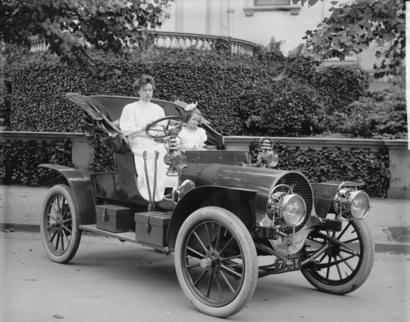
\includegraphics[width=\linewidth]{sample-franklin}
  \caption{1907 Franklin Model D roadster. Photograph by Harris \&
    Ewing, Inc. [Public domain], via Wikimedia
    Commons. (\url{https://goo.gl/VLCRBB}).}
\end{figure}

Your figures should contain a caption which describes the figure to
the reader. Figure captions go below the figure. Your figures should
also include a description suitable for screen readers, to
assist the visually-challenged to better understand your work.

Figure captions are placed below the figure.

\section{Citations and Bibliographies}

The use of Bib\TeX{} for the preparation and formatting of one's
references is strongly recommended. Authors' names should be complete
--- use full first names (``Donald E. Knuth'') not initials
(``D. E. Knuth'') --- and the salient identifying features of a
reference should be included: title, year, volume, number, pages,
article DOI, etc.

The bibliography is included in your source document with these two
commands, placed just before the \verb|\end{document}| command:
\begin{minted}{latex}
\bibliography{bibfile}
\end{minted}
where ``\verb|bibfile|'' is the name, without the ``\verb|.bib|''
suffix, of the Bib\TeX{} file.


\subsection{Some examples}

A paginated journal article \cite{Abril07}, an enumerated journal
article \cite{Cohen07}, a reference to an entire issue
\cite{JCohen96}, a monograph (whole book) \cite{Kosiur01}, a
monograph/whole book in a series (see 2a in spec. document)
\cite{Harel79}, a divisible-book such as an anthology or compilation
\cite{Editor00} followed by the same example, however we only output
the series if the volume number is given \cite{Editor00a} (so series
should not be present since it has no vol. no.), a chapter in a
divisible book \cite{Spector90}, a chapter in a divisible book in a
series \cite{Douglass98}, a multi-volume work as book \cite{Knuth97},
an article in a proceedings (of a conference, symposium, workshop for
example) (paginated proceedings article) \cite{Andler79}, a
proceedings article with all possible elements \cite{Smith10}, an
example of an enumerated proceedings article \cite{VanGundy07}, an
informally published work \cite{Harel78}, a doctoral dissertation
\cite{Clarkson85}, a master's thesis: \cite{anisi03}, an online
document / world wide web resource \cite{Thornburg01, Ablamowicz07,
  Poker06}, a video game (Case 1) \cite{Obama08} and (Case 2)
\cite{Novak03} and \cite{Lee05} and (Case 3) a patent
\cite{JoeScientist001}, work accepted for publication \cite{rous08},
prolific author \cite{SaeediMEJ10} and \cite{SaeediJETC10}. Other
cites might contain `duplicate' DOI and URLs (some SIAM articles)
\cite{Kirschmer:2010:AEI:1958016.1958018}. Multi-volume works as books
\cite{MR781536} and \cite{MR781537}. A couple of citations with DOIs:
\cite{2004:ITE:1009386.1010128,Kirschmer:2010:AEI:1958016.1958018}. Online
citations: \cite{TUGInstmem, Thornburg01, R, UMassCitations}.

\section{Acknowledgments}

Identification of funding sources and other support, and thanks to
individuals and groups that assisted in the research and the
preparation of the work should be included in an acknowledgment
section, which is placed just before the reference section in your
document.

This section has a special environment:
\begin{minted}{latex}
\begin{acknowledgments}
  These are different acknowledgments.
\end{acknowledgments}
\end{minted}
so that the information contained therein can be more easily collected
during the article metadata extraction phase, and to ensure
consistency in the spelling of the section heading.

Authors should not prepare this section as a numbered or unnumbered
{\verb|\section|}; please use the ``{\verb|acknowledgments|}'' environment.

\section{Appendices}

If your work needs an appendix, add it before the
``\verb|\end{document}|'' command at the conclusion of your source
document.

Start the appendix with the ``\verb|appendix|'' command:
\begin{minted}{latex}
\appendix
\end{minted}
and note that in the appendix, sections are lettered, not
numbered.

%%
%% The acknowledgments section is defined using the "acknowledgments" environment
%% (and NOT an unnumbered section). This ensures the proper
%% identification of the section in the article metadata, and the
%% consistent spelling of the heading.
\begin{acknowledgments}
  Thanks to the developers of ACM consolidated LaTeX styles
  \url{https://github.com/borisveytsman/acmart} and to the developers
  of Elsevier updated \LaTeX{} templates
  \url{https://www.ctan.org/tex-archive/macros/latex/contrib/els-cas-templates}.
\end{acknowledgments}

%%
%% Define the bibliography file to be used
% \bibliography{sample-ceur}

\begin{thebibliography}{99}

\bibitem{hogan} Aidan Hogan, Eva Blomqvist, Michael Cochez, Claudia D’Amato \emph{et al}. Knowledge Graphs. \url{https://arxiv.org/abs/2003.02320v5}
\bibitem{lgd} Claus Stadler, Jens Lehmann, Konrad Höffner, Sören Auer. LinkedGeoData: A core for a web of spatial open data. Semantic Web 3 (2012) 333–354. \doi{10.3233/SW-2011-0052}

\bibitem{iwaniak1} Adam Iwaniak, Iwona Kaczmarek, Marek Strzelecki, Jaromar Lukowicz, Piotr Jankowski. Enriching and improving the quality of linked data with GIS. \doi{10.1515/geo-2016-0c020}

\bibitem{iwaniak17} Adam Iwaniak, Marta Leszczuk, Marek Strzelecki, Francis Harvey, Iwona Kaczmarek. A Novel Approach for Publishing Linked Open Geodata from National Registries with the Use of Semantically Annotated Context Dependent Web Pages. International Journal of Geo-Information. 6, 252, 2017. \doi{10.3390/ijgi6080252}

\bibitem{abid} Tarek Abid, Hafed Zarzour. Integrating Linked Open Data in Geographical
Information System. International Conference on Information Technology for Organization Development. 2014.

\bibitem{geolink} Michelle Cheatham, Adila Krisnadhi, Reihaneh Amini, Pascal Hitzler, \emph{et al} (2018) The GeoLink knowledge graph, Big Earth Data, 2:2, 131-143, \doi{10.1080/20964471.2018.1469291}

\bibitem{lunina} Oksana V. Lunina.  The digital map of the pliocene quaternary crustal faults in the southern east siberia and the adjacent northern Mongolia. Geodynamics \& Tectonophysics. 2016. 7(3):407-434. \doi{10.5800/GT-2016-7-3-0215}
\bibitem{afs} Server activefaults.ru
\bibitem{foss} Mathias Leidig, Richard Teeuw. Free software: A review, in the context of disaster management. 2015. International Journal of Applied Earth Observation and Geoinformation,
Vol.~42, pp.~49-56, ISSN 0303-2434, \doi{10.1016/j.jag.2015.05.012}.
\end{thebibliography}


%%
%% If your work has an appendix, this is the place to put it.
\appendix

\section{Online Resources}


The sources for the ceur-art style are available via
\begin{itemize}
\item \href{https://github.com/yamadharma/ceurart}{GitHub},
% \item \href{https://www.overleaf.com/project/5e76702c4acae70001d3bc87}{Overleaf},
\item
  \href{https://www.overleaf.com/latex/templates/template-for-submissions-to-ceur-workshop-proceedings-ceur-ws-dot-org/pkfscdkgkhcq}{Overleaf
    template}.
\end{itemize}

\end{document}

%%
%% End of file

%%% Local Variables:
%%% mode: latex
%%% TeX-master: t
%%% End:
